\chapter{Testing the application and experimental results}

\section{Deployment and Configuration}

The application leverages a modern cloud-native deployment strategy, hosted entirely 
within the Microsoft Azure ecosystem. Because the backend is built using a decoupled 
microservices topology, each service is isolated, configured, and deployed independently 
to simplify environment management.

The solution is deployed using a straightforward, manual approach on Azure:
\begin{itemize}
    \item \textbf{Frontend Deployment:} The React single-page application is compiled into
    static assets and served directly from an Azure Blob Storage container, provisioned
    under a dedicated Azure Storage Account with static website hosting enabled.
    \item \textbf{Backend Microservices:} Both the main API application
    layer (\texttt{DailyPlanService} and \newline\texttt{UserManagementService}) and the
    computational engine (\texttt{OptimizerService}) are packaged as Docker images, built
    locally and pushed to an Azure Container Registry (ACR), then deployed as individual
    Azure Container Apps within a shared Container App Environment.
    \item \textbf{Database Infrastructure:} Relational and transactional user records are 
    mapped to a cloud-managed Azure SQL Database instance, while the optimizer reads 
    directly from its companion embedded SQLite database file located inside its 
    container file system.
\end{itemize}

Configuration management relies on environment variables injected at runtime by the Azure
Container Apps host, eliminating hardcoded credentials from the codebase. The key
parameters configured per service are:
\begin{itemize}
    \item \texttt{ConnectionStrings:DefaultConnection}: The connection string pointing to
    the cloud-managed Azure SQL Database instance, shared by both \texttt{DailyPlanService}
    and \texttt{UserManagementService}.
    \item \texttt{Jwt:Key}: A 256-bit symmetric secret used by the \texttt{TokenService}
    to sign and validate session tokens.
    \item \texttt{Cors:AllowedOrigins}: The public URL of the frontend Azure Blob Storage
    static website, used to restrict cross-origin requests to the known client origin.
    \item \texttt{Optimizer:Url}: The internal URI of the
    \texttt{OptimizerService} container, configured exclusively on \texttt{DailyPlanService}
    to route meal optimization requests to the computational engine.
\end{itemize}

\section{System Testing (Hardware and Software)}

System testing was executed to verify the seamless interaction between the 
decoupled client-side application, the backend microservices, and the hybrid 
database layer. The testing methodology focused on validating complete 
functional flows, ensuring that security boundaries remain intact, and 
verifying data synchronization across services.

\subsection{Testing Environment and Infrastructure}
Testing was carried out across both local and cloud environments:
\begin{itemize}
    \item \textbf{Software Environment:} Backend services run inside Linux-based
    Docker containers on the .NET 10 runtime. Client-side testing was performed
    in a Chromium-based browser against the React production build.
    \item \textbf{Infrastructure:} Local testing verified inter-container
    communication on a development machine, while final validation was performed
    against the live deployment on Azure Container Apps.
\end{itemize}

\subsection{End-to-End Integration Flow Verification}
To ensure the reliability of the system, testing was structured around the core end-to-end 
user journeys defined during the high-level design phase. These flows were mapped directly 
against the architectural sequence diagrams to verify that request routing, validation, 
and token evaluation occur in the correct logical order:

\begin{enumerate}
    \item \textbf{Authentication and Onboarding Flow:} Testing verified the full new-user
    path: registering an account, logging in, and completing the initial profile setup form.
    The form captures height, weight, sex, activity level, and goal, which are persisted to
    the database and associated with the authenticated user. Login was confirmed to return a
    short-lived JWT access token held in memory and a long-lived refresh token issued as an
    HttpOnly cookie. Access to protected routes was verified to be blocked for unauthenticated
    requests.
    \item \textbf{Meal Plan Generation Flow:} Testing verified the full generation cycle
    triggered when the user requests an AI-generated plan. The \texttt{DailyPlanService}
    receives the request, calculates the user's target calorie intake from their stored
    profile, and forwards that value to the \newline\texttt{OptimizerService}, which 
    returns a structured meal plan. The response is surfaced to the user as a preview, 
    from which they can either confirm and save the plan to their daily log or discard 
    it and trigger a new generation cycle.
    \item \textbf{Token Refresh Flow:} Testing verified the silent token renewal mechanism.
    When an API request returns a 401 due to an expired access token, the frontend
    automatically issues a \texttt{POST /api/user/refresh} request carrying the HttpOnly
    refresh token cookie. The UserManagementService validates the token, 
    queries the associated user, deletes the old refresh token, and persists a newly rotated 
    one. A fresh JWT access token and updated refresh cookie are returned, after which the 
    frontend transparently retries the original request — all without requiring the user to
    re-authenticate.
    \item \textbf{Meal Plan CRUD Operations:} Testing validated that manually adding,
    updating, or deleting individual food items within an active meal slot correctly
    persists state changes to the database without causing data corruption or
    macro-nutrient desynchronization.
\end{enumerate}

\subsection{User Interface and Functional Validation}
The following screenshots illustrate the key interface states exercised during functional
validation, covering the onboarding flow, meal plan generation, daily tracking, and
plan editing.

\begin{figure}[htbp]
    \centering
    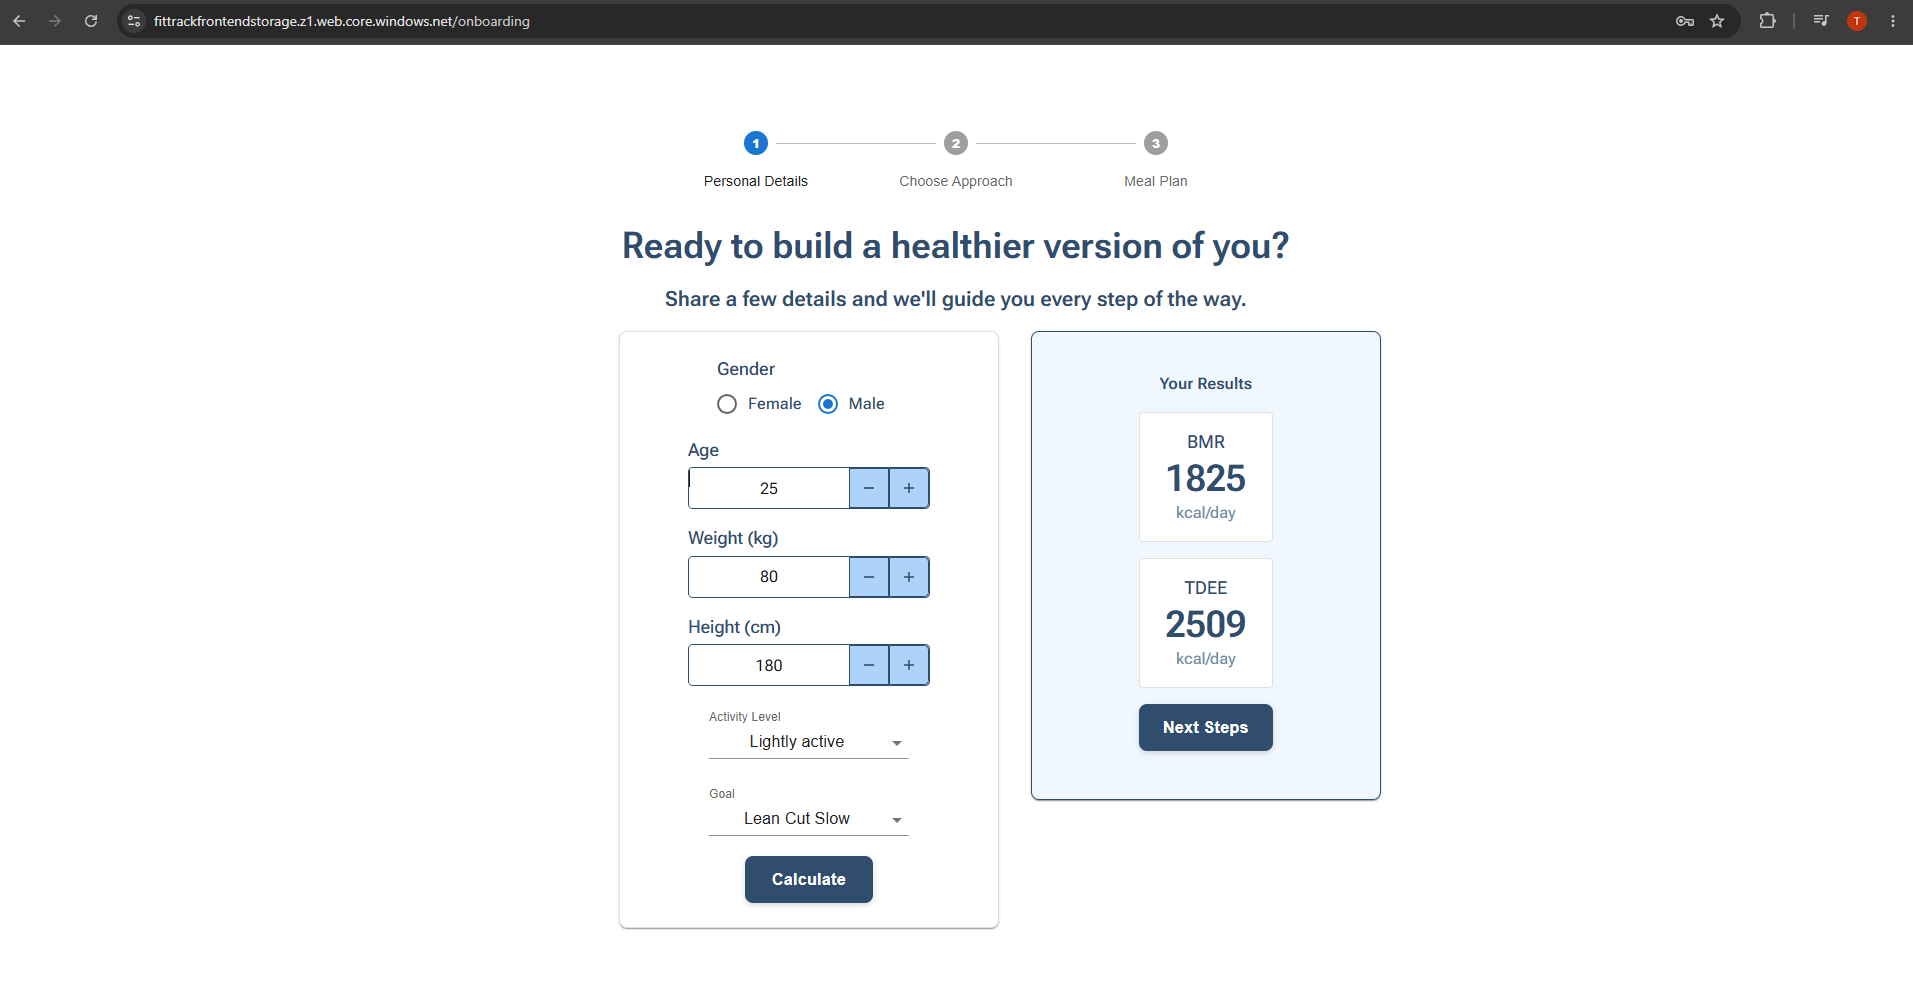
\includegraphics[width=0.9\textwidth]{continut/capitol4/screenshots/OnboardingFlow.png}
    \caption{User profile setup form capturing height, weight, sex, activity level, and goal.}
    \label{fig:onboarding}
\end{figure}

Figure~\ref{fig:onboarding} shows the onboarding form presented immediately after login.
The submitted values are persisted to the database and used as the basis for all
subsequent calorie and macro-nutrient calculations.

\begin{figure}[htbp]
    \centering
    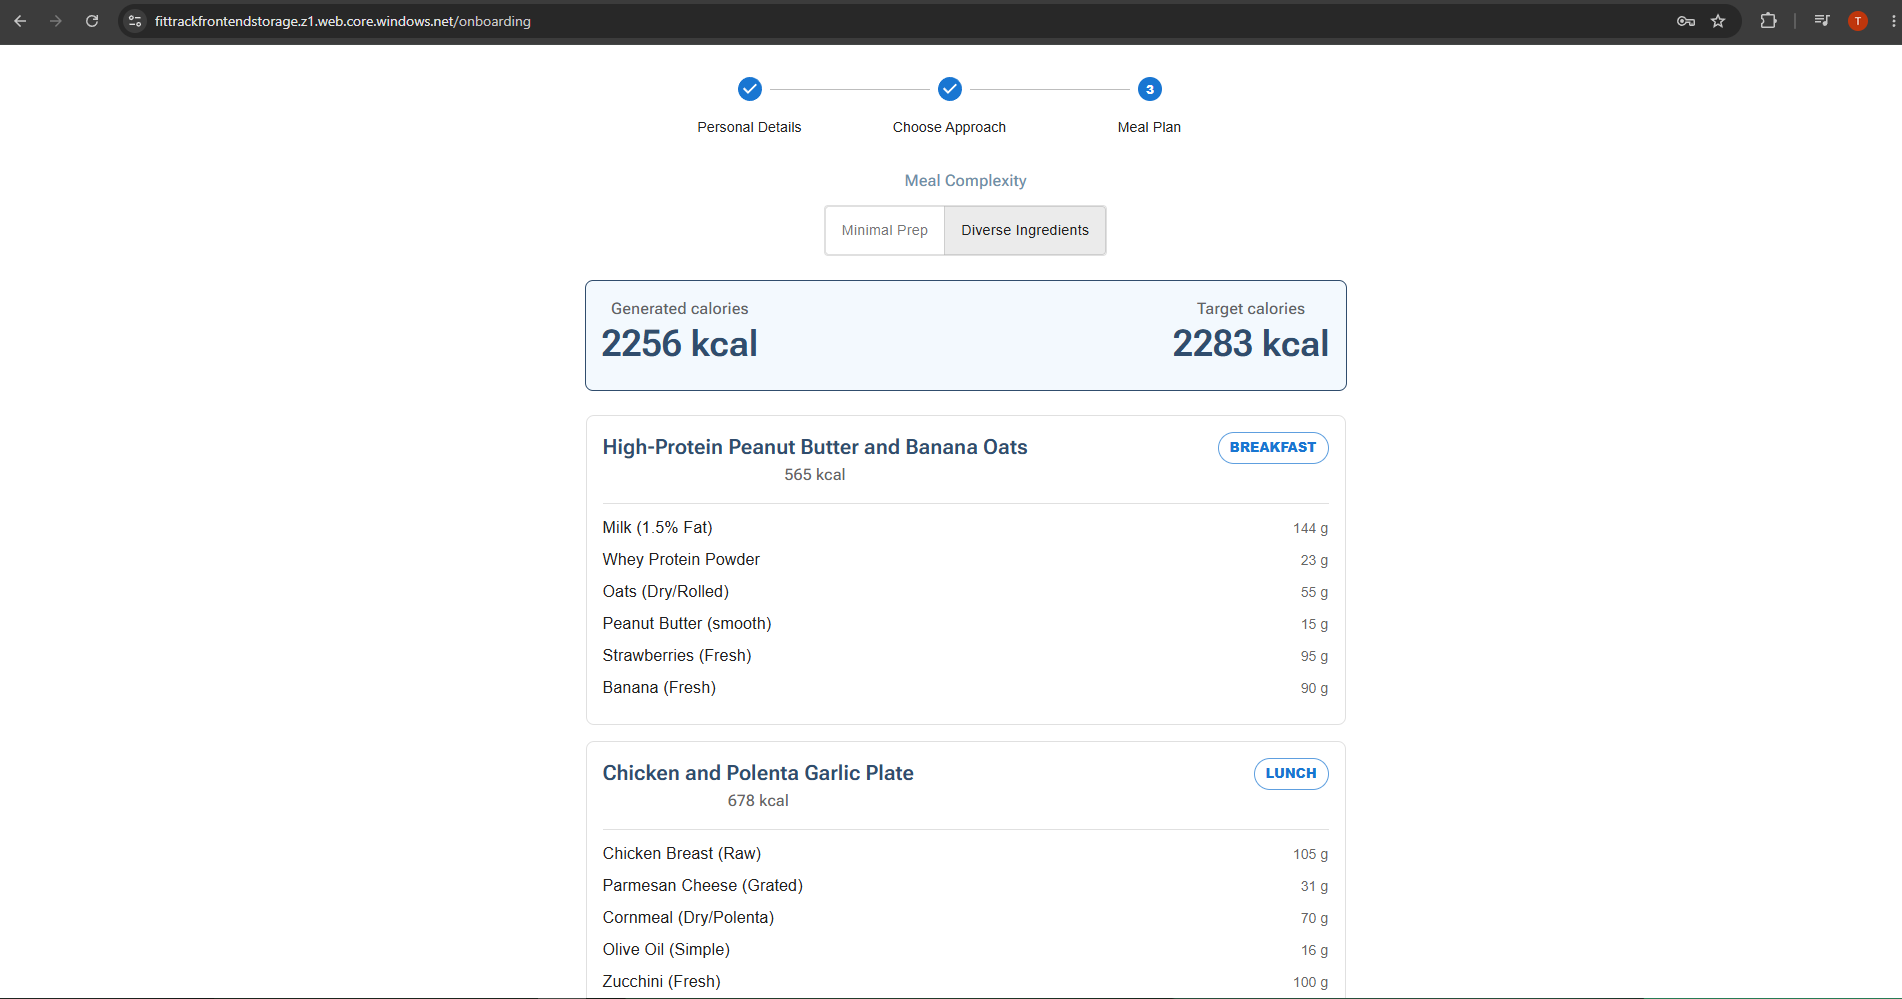
\includegraphics[width=0.9\textwidth]{continut/capitol4/screenshots/MealPreview.png}
    \caption{Read-only meal plan preview returned by the optimizer, with accept and regenerate options.}
    \label{fig:meal_preview}
\end{figure}

Figure~\ref{fig:meal_preview} shows the generated meal plan preview. The view is
read-only — the user can either confirm the plan and add it to their daily log, or
discard it and request a new generation cycle.

\begin{figure}[htbp]
    \centering
    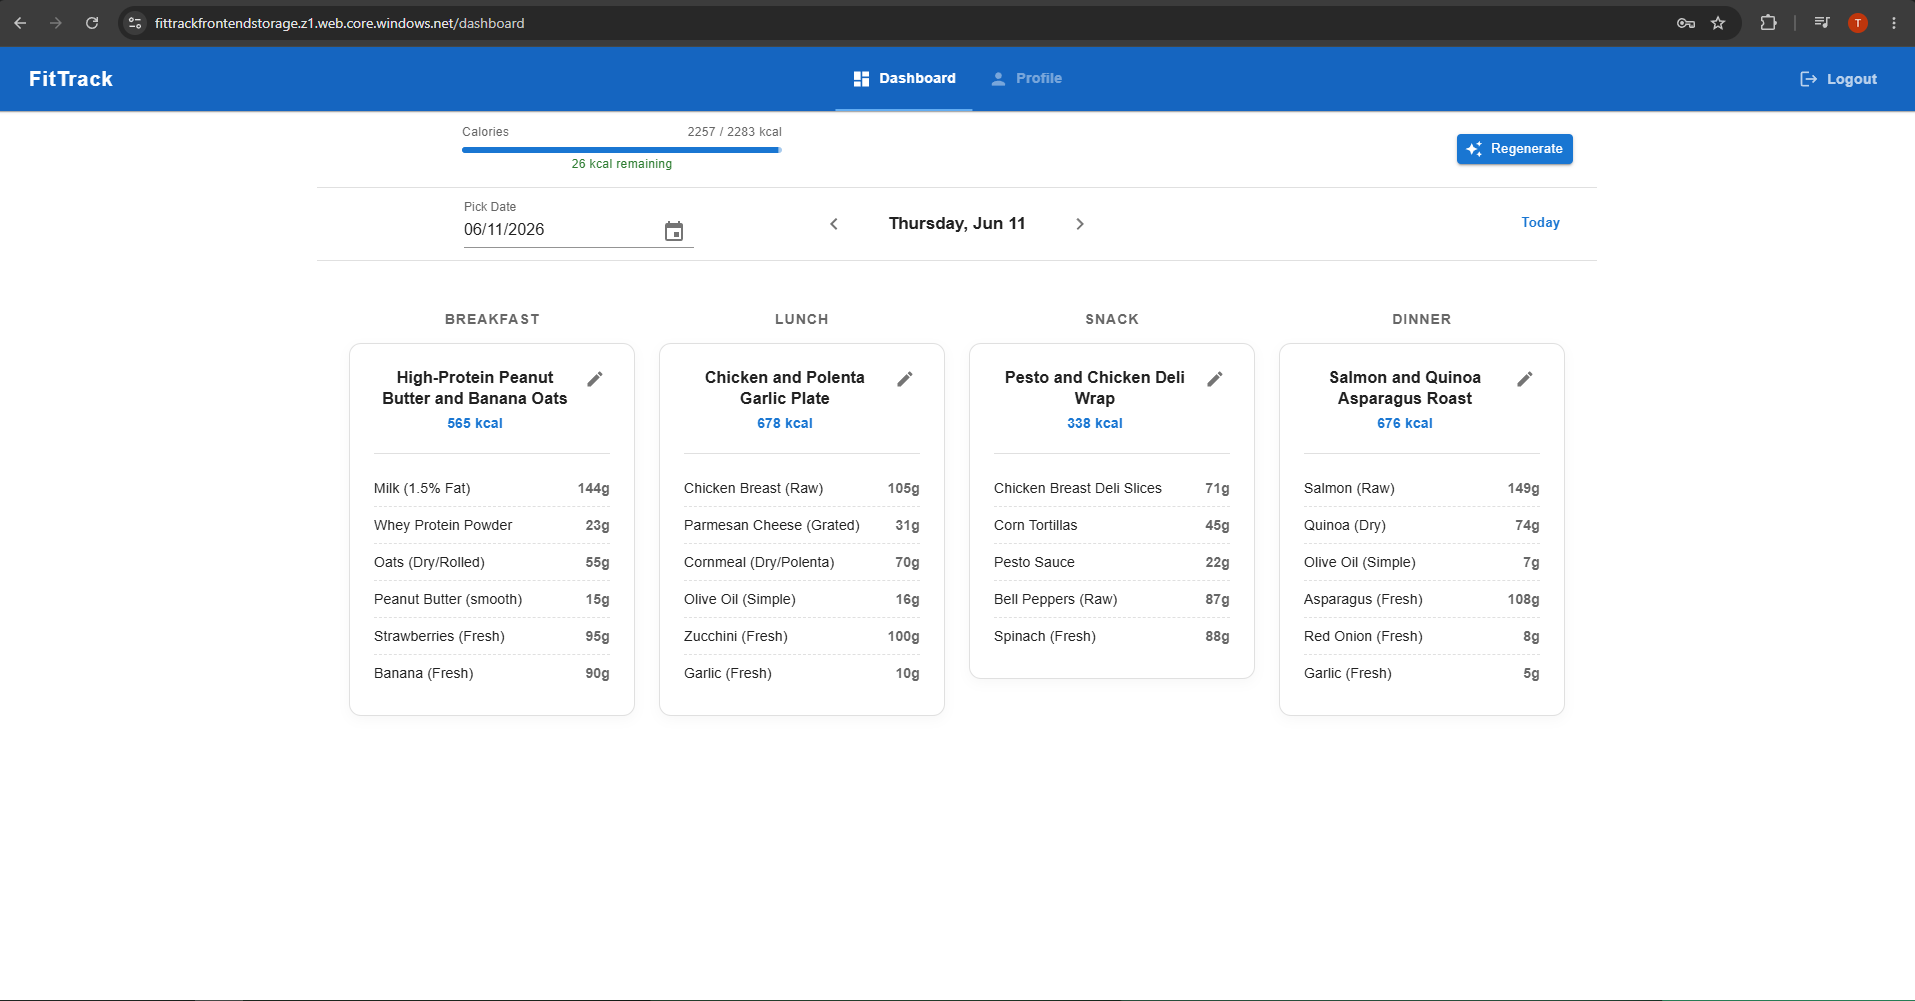
\includegraphics[width=0.9\textwidth]{continut/capitol4/screenshots/Dashboard.png}
    \caption{Main dashboard displaying the daily macro-nutrient progress and logged meals.}
    \label{fig:dashboard}
\end{figure}

Figure~\ref{fig:dashboard} shows the main dashboard, where macro-nutrient progress bars
update in real time as meals are logged throughout the day.

\begin{figure}[htbp]
    \centering
    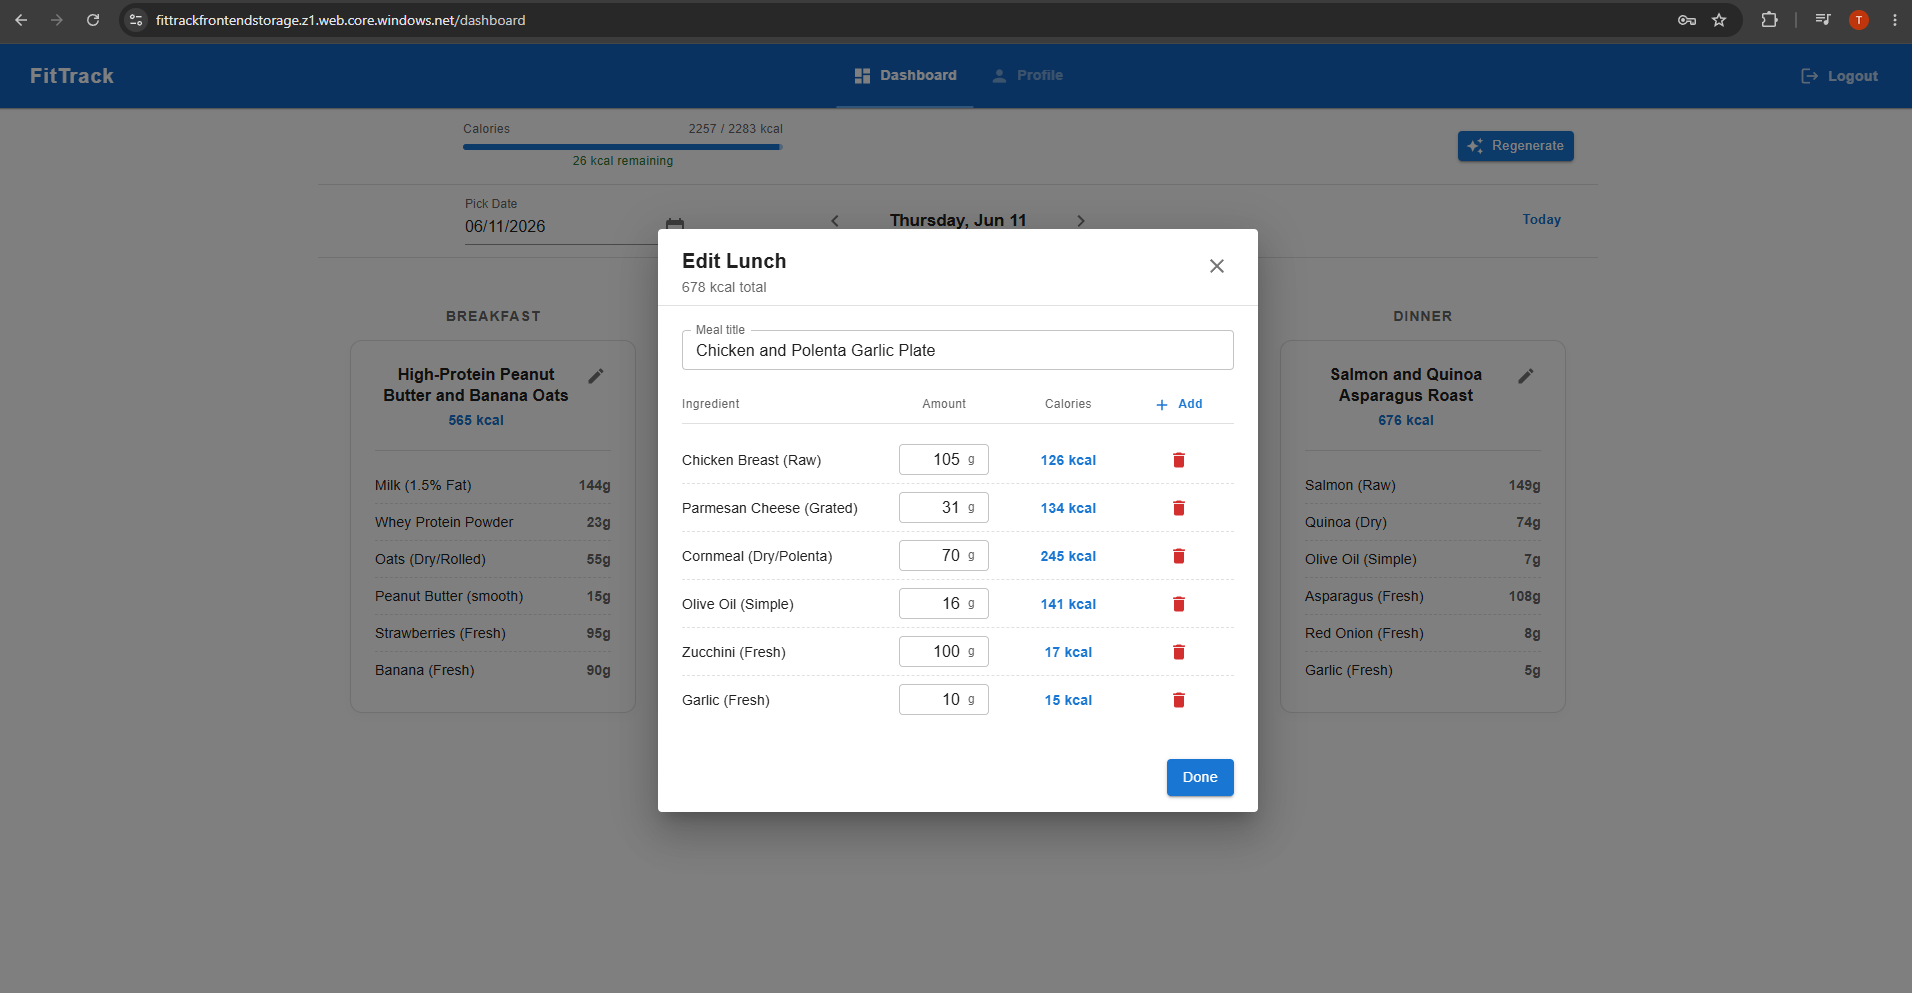
\includegraphics[width=0.9\textwidth]{continut/capitol4/screenshots/EditDailyPlan.png}
    \caption{Daily plan editing view with inline ingredient management and live macro recalculation.}
    \label{fig:edit_plan}
\end{figure}

Figure~\ref{fig:edit_plan} shows the plan editing view, where the user can add, edit,
or remove individual ingredients within a meal slot, rename the meal, and observe
calorie and macro totals recalculate immediately with each change.

\section{Performance, Reliability, and Scalability}

All three backend services are deployed as Azure Container Apps within a shared Container
App Environment, running on shared-tier cloud hardware. The resource consumption observed
during live testing reflects the lightweight nature of the workload.

\begin{figure}[htbp]
    \centering
    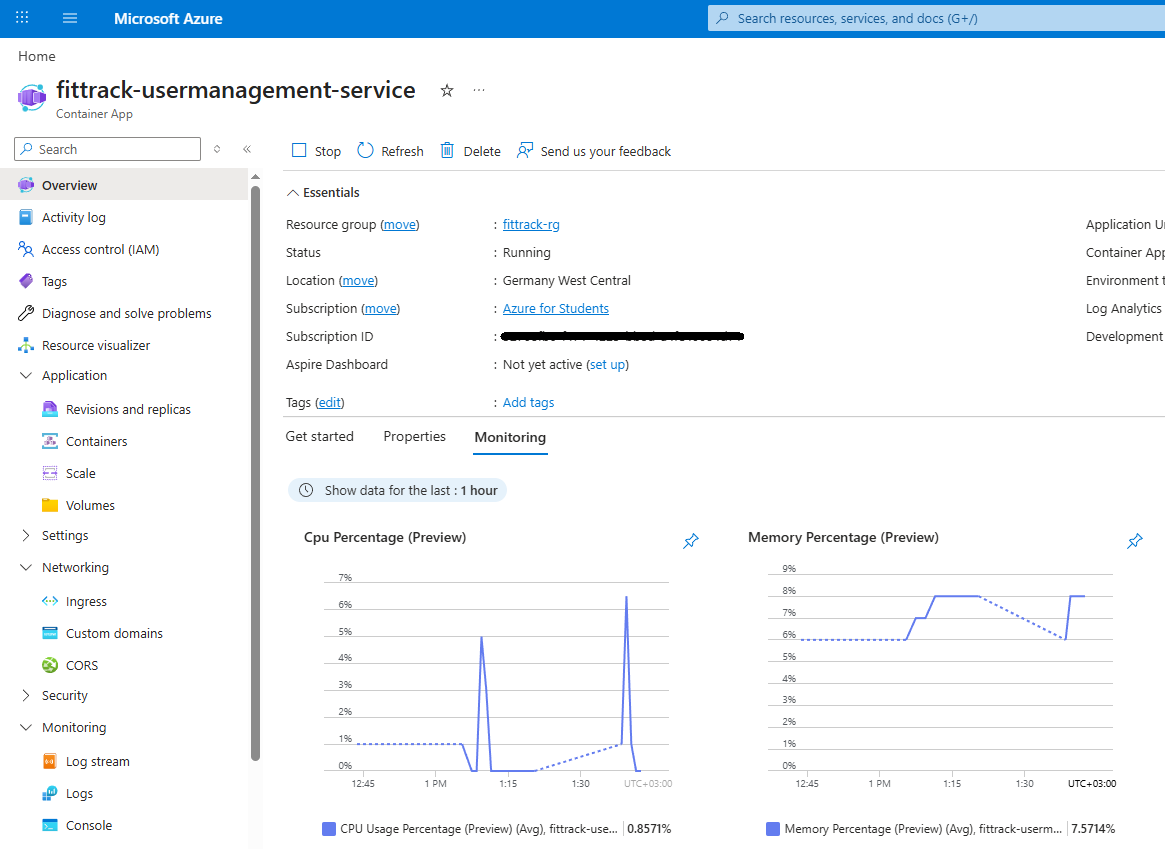
\includegraphics[width=0.9\textwidth]{continut/capitol4/screenshots/UserManagementUsage.png}
    \caption{CPU and memory usage for \texttt{UserManagementService} under live traffic.}
    \label{fig:usage_usermgmt}
\end{figure}

\begin{figure}[htbp]
    \centering
    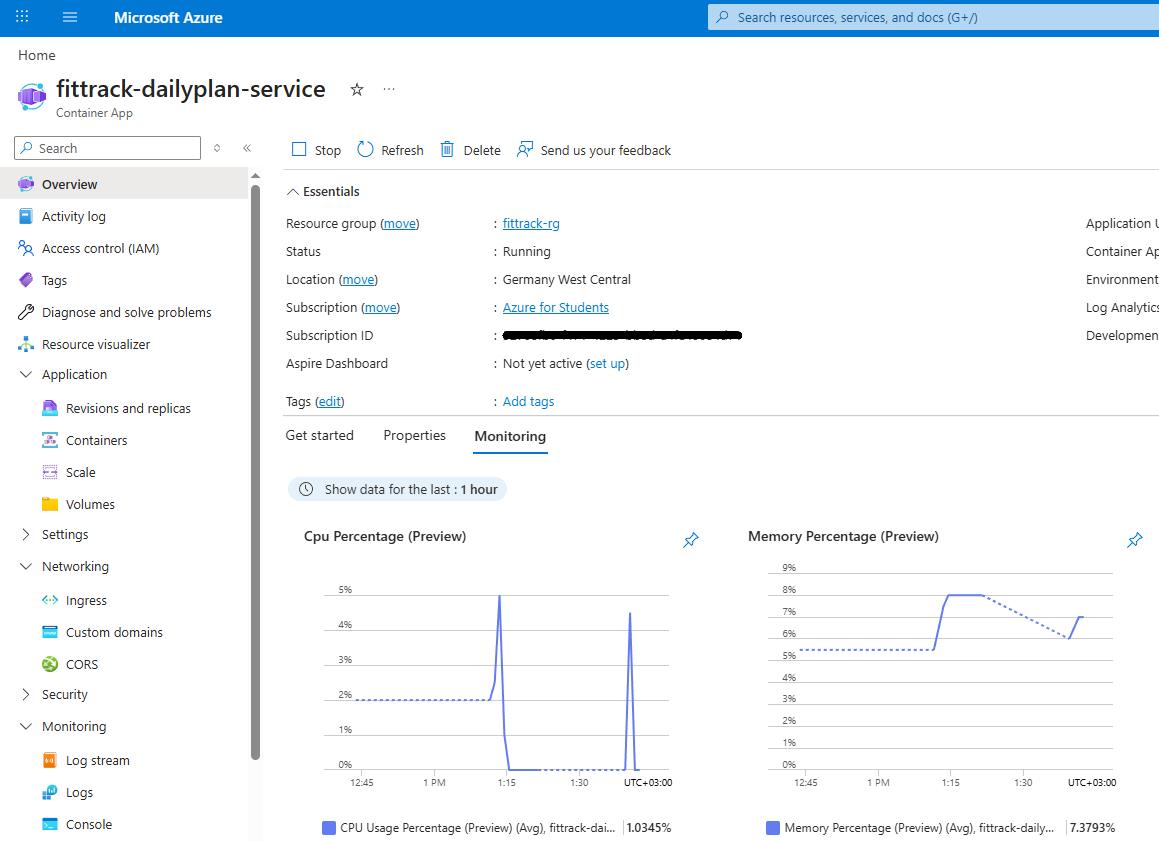
\includegraphics[width=0.9\textwidth]{continut/capitol4/screenshots/DailyPlanUsage.png}
    \caption{CPU and memory usage for \texttt{DailyPlanService} under live traffic.}
    \label{fig:usage_dailyplan}
\end{figure}

As shown in Figures~\ref{fig:usage_usermgmt} and~\ref{fig:usage_dailyplan}, both
\texttt{UserManagementService} and \texttt{DailyPlanService} maintain a steady memory footprint
of approximately 7.5\% at idle, with CPU spiking briefly to 5--6\% when a request is
processed and returning immediately to near-zero baseline. This confirms that neither
service sustains load between requests.

\begin{figure}[htbp]
    \centering
    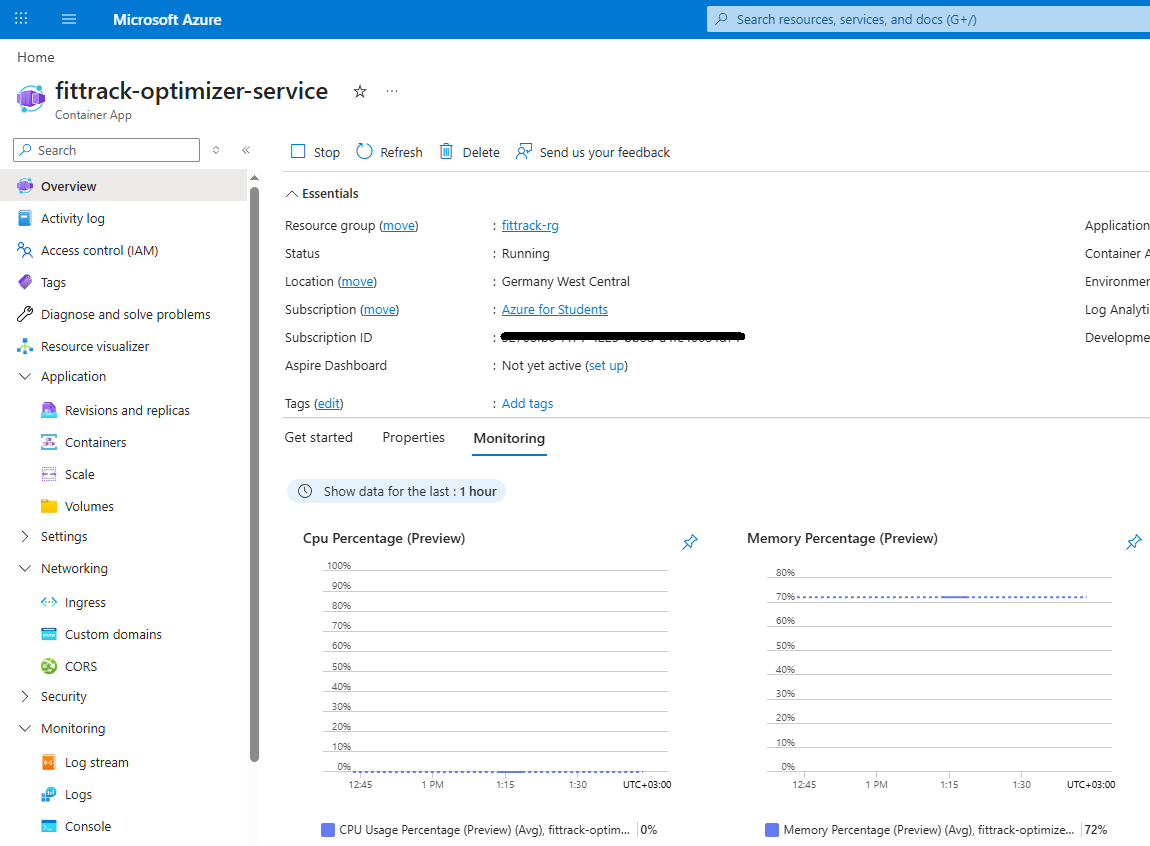
\includegraphics[width=0.9\textwidth]{continut/capitol4/screenshots/OptimizerUsage.png}
    \caption{CPU and memory usage for \texttt{OptimizerService} at steady state.}
    \label{fig:usage_optimizer}
\end{figure}

Figure~\ref{fig:usage_optimizer} shows a different profile for the \texttt{OptimizerService}.
Its memory usage sits consistently around 70\%, which is expected: the embedded SQLite
database is loaded into memory at container startup and held resident for the lifetime of
the instance. CPU usage remains near zero between optimization requests, as the service
performs no background computation.

From a reliability standpoint, each service is isolated within its own container, meaning
a failure in one does not directly affect the others. Token rotation on every refresh cycle
limits the exposure window of any compromised credential. The stateless design of both API
services means horizontal scaling can be applied per container independently should traffic
demand increase.

\newpage
\section{Test Data and Experimental Results}

This section describes the dataset used to populate the optimizer's read-only database
and presents the experimental results obtained by running the meal plan generation
algorithm across a representative set of user profiles.

\subsection{Test Data}

The \texttt{OptimizerService} relies on a read-only SQLite database bundled directly
inside its container image. The dataset was assembled from two sources and populated
using Python scripts prior to building the container.

Nutritional data for individual ingredients was sourced from a CSV file containing
per-100g macronutrient values (calories, protein, fats, carbohydrates) for each food
item. A Python script parsed the file and inserted the records into the ingredients
table of the SQLite database.

Meal definitions were sourced from a separate text file listing recipe names alongside
their constituent ingredients. A second Python script parsed this file and populated
the meals and meal-ingredients tables, linking each recipe to its ingredient entries
by identifier. The resulting database ships as a static artifact embedded in the
\texttt{OptimizerService} container image and is never modified at runtime.

\subsection{Experimental Results}

To evaluate the accuracy of the meal plan generation algorithm, the optimizer was
tested across six user profiles spanning all three activity groups and a range of
dietary goals. For each profile, the target calorie intake was calculated by
\texttt{DailyPlanService} and forwarded to \texttt{OptimizerService}, which returned
a structured daily meal plan. The top-level response includes a \texttt{targetCalories}
field alongside the \texttt{actualCalories} delivered by the generated plan, allowing
the deviation to be measured directly.

\begin{table}[htbp]
    \centering
    \begin{tabular}{|l|l|r|r|r|}
        \hline
        \textbf{Group} & \textbf{Goal} & \textbf{Target (kcal)} & \textbf{Actual (kcal)} & \textbf{Deviation} \\
        \hline
        G1 & Lose Fat (Aggressive) & 1870 & 1846 & 1.28\% \\
        G1 & Lean Cut (Slow)       & 1794 & 1776 & 1.00\% \\
        G2 & Maintain Form         & 2600 & 2575 & 0.96\% \\
        G2 & Lean Bulk             & 2646 & 2626 & 0.76\% \\
        G3 & Maintain Form         & 2500 & 2468 & 1.28\% \\
        G3 & Power Bulk            & 3564 & 3539 & 0.70\% \\
        \hline
    \end{tabular}
    \caption{Optimizer calorie deviation across activity groups and dietary goals.}
    \label{tab:optimizer_results}
\end{table}

As shown in Table~\ref{tab:optimizer_results}, the optimizer consistently delivers
meal plans within 1.3\% of the target calorie intake across all tested profiles. The
deviation is inherent to the constraint that ingredient amounts must be expressed as
discrete gram values — the optimizer cannot fractionally adjust portions to close the
remaining gap exactly. Notably, the deviation tends to decrease at higher calorie
targets, where the larger ingredient budget provides more room to approximate the
target closely.

The following is a representative excerpt of the API response returned by the
\texttt{OptimizerService} for one of the tested profiles, illustrating the top-level
structure and a single meal entry:

\begin{verbatim}
{
  "targetCalories": 2646,
  "actualCalories": 2626,
  "meals": [
    {
      "category": "LUNCH",
      "title": "Turkey Breast and Quinoa Power Bowl",
      "mealId": 35,
      "calories": 630,
      "ingredients": [ ... ],
      "error": 9.18e-10
    },
    ...
  ]
}
\end{verbatim}

The per-meal \texttt{error} field is the residual reported by the SLSQP solver and
reflects numerical precision rather than a meaningful deviation — values in the range
of $10^{-10}$ to $10^{-15}$ indicate that the optimizer converged to a solution
satisfying its constraints to machine precision.

Overall, the results confirm that the system behaves correctly across the full range of
supported user profiles. The optimizer produces nutritionally consistent meal plans with
a maximum calorie deviation of 1.28\%, which in absolute terms amounts to at most 32 kcal
— well within the natural variance introduced by home cooking and portion estimation.
The end-to-end flows validated in this chapter demonstrate that the application meets
its functional requirements from authentication through to daily plan management.
